% Projekt 5
% Typografie a publikovani
% Autor: Nikola Valesova
% Datum: 1. 5. 2016

\documentclass{beamer}
\setbeamertemplate{navigation symbols}{}
\usepackage[czech]{babel}
\usepackage[utf8]{inputenc}
\usepackage{times}
\usepackage{tipa}
\usetheme{Montpellier}
\beamersetuncovermixins{\opaqueness<1>{25}}{\opaqueness<2->{15}}

\title{Dějiny typografie}
\author{Nikola Valešová}
\institute{Fakulta informačních technologií\\
Vysoké učení technické v~Brně}
\date{\today}

\begin{document}

\begin{frame}
\titlepage
\logo{
\includegraphics[height=1.5cm]{logo2.eps}}
\begin{center}
\insertlogo
\end{center}
\end{frame}

\begin{frame}
\frametitle{Obsah}
\tableofcontents
\end{frame}

\section{Úvod}
\subsection{Co je to typografie}
\begin{frame}\frametitle{Co je to typografie}
\begin{itemize}
\item Umělecko-technický obor \pause
\item Zabývá se tiskovým písmem a~jeho úpravou \pause
\item Cílem je usnadnit čtení a~zefektivnit vnímání čteného textu \pause
\item Dva základní směry \pause
\begin{enumerate}
\item{Mikrotypografie} \pause
\item{Makrotypografie} \pause
\end{enumerate}
\item{Název odvozen z~řeckého výrazu pro formu či dojem}
\end{itemize} 
\end{frame}

\section{Historie} 
\subsection{Počátky vzniku typografie}
\begin{frame}\frametitle{Počátky vzniku typografie}
\begin{columns}
\begin{column}{7cm}
\begin{itemize}
\item	Počátek dějin typografie kolem poloviny 15. století \pause
\item	Základním kamenem vznik knihtisku \pause
\item	Přelom 15. a~16. století\,--\,vznik dvou základních forem latinského písma \pause
\begin{enumerate}
\item{Humanistické} \pause
\item{Novogotické}
\end{enumerate}
\end{itemize}
\end{column}
\begin{column}{6cm}
\begin{figure}
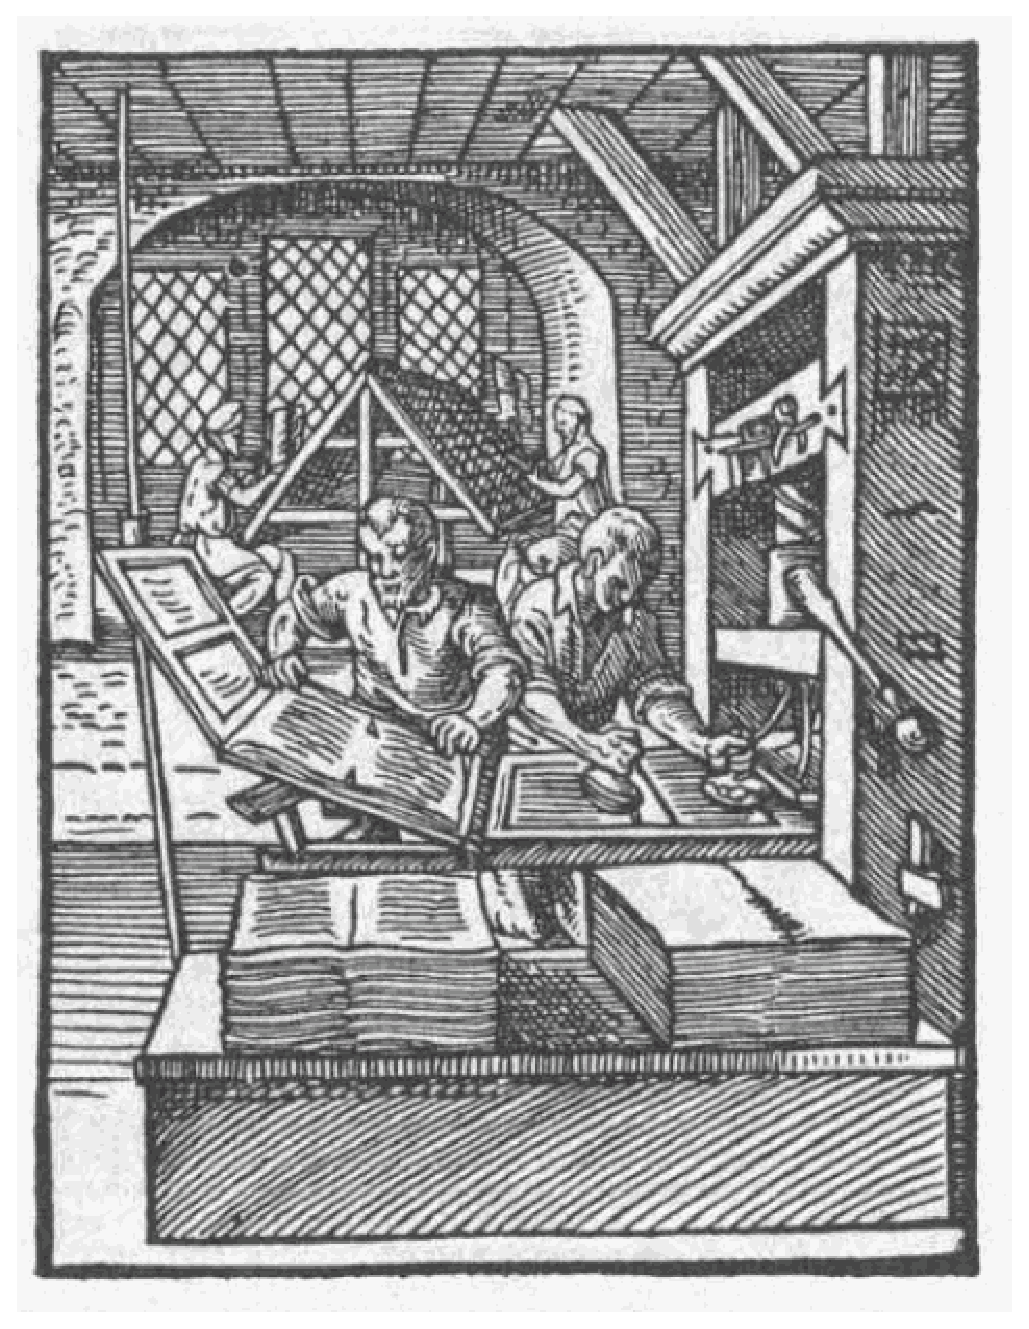
\includegraphics[scale=0.18]{knihtisk.eps} 
\caption{Knihtisk v~16. století}
\end{figure}
\end{column}
\end{columns}
\end{frame}

\subsection{Vývoj novogotického písma}
\begin{frame}\frametitle{Vývoj novogotického písma}
\begin{itemize}
\item Novogotické písmo odvozeno od gotického \pause
\item Postupně se vyvinuly tři základní druhy novogotického písma \pause
\begin{enumerate}
\item{Kreslené novogotické písmo} \pause
\item{Novogotické polokurzívní písmo} \pause
\item{Novogotické kurzívní písmo} \pause
\end{enumerate}
\item Novogotická písma se používala až do poloviny 19. století \pause
\item Od roku 1941 přechod na písmo humanistické
\end{itemize} 
\end{frame}

\subsection{Další vývoj typografie}
\begin{frame}\frametitle{Další vývoj typografie}
\begin{itemize}
\item Polovina 15. století\,--\,odpor proti novogotickému písmu, vznik antikvy \pause
\item Antikva nejprve používána pouze omezeně, později se rozšířila do většiny zemí Evropy \pause
\item 1550\,--\,konec užívání kurzívy na běžný text \pause
\item Rokoko\,--\,využívání grafických odrážek a~ornamentálních dekorací \pause
\item{Klasicismus\,--\,nárůst technického charakteru písma, užší písmo s~přímějším sklonem}
\end{itemize} 
\end{frame}


\section{Osobnosti}
\subsection{Nejznámější světoví typografové} 
\begin{frame}
\frametitle{Nejznámější světoví typografové}
\begin{columns}
\begin{column}{5cm}
\begin{itemize}
\item<1-> William Caslon
\item<3-> Giambattista Bodoni
\end{itemize}
\vspace{3cm} 
\end{column}
\begin{column}{6cm}
\begin{overprint}
\includegraphics<2>[height=5cm]{Caslon.eps}
\includegraphics<4>[height=5cm]{Bodoni.eps}
\end{overprint}
\end{column}
\end{columns}
\end{frame}

\subsection{Nejznámější čeští typografové}
\begin{frame}
\frametitle{Nejznámější čeští typografové}
\begin{columns}
\begin{column}{5cm}
\begin{itemize}
\item<1-> Daniel Adam z~Veleslavína
\item<3-> Mikoláš Aleš
\item<5-> Adolf Kašpar
\end{itemize}
\vspace{3cm} 
\end{column}
\begin{column}{6cm}
\begin{overprint}
\includegraphics<2>[height=5cm]{Adam.eps}
\includegraphics<4>[height=5cm]{Ales.eps}
\includegraphics<6>[height=5cm]{Kaspar.eps}
\end{overprint}
\end{column}
\end{columns}
\end{frame}

\section{Použité zdroje}
\begin{frame}\frametitle{Použité zdroje}
\begin{itemize}
\item Typografie\,--\,Wikipedie\\
\texttt{https://cs.wikipedia.org/wiki/Typografie}
\item Co je Typografie\,\textpipe\,Adaptic\\
\texttt{www.adaptic.cz/znalosti/slovnicek/typografie}
\item Beamer\,--\,ShareLaTeX, Online LaTeX Editor\\
\texttt{https://www.sharelatex.com/learn/Beamer} 
\end{itemize}
\end{frame}

\end{document}
